\section{Results}
\begin{figure*}[t]
\centering
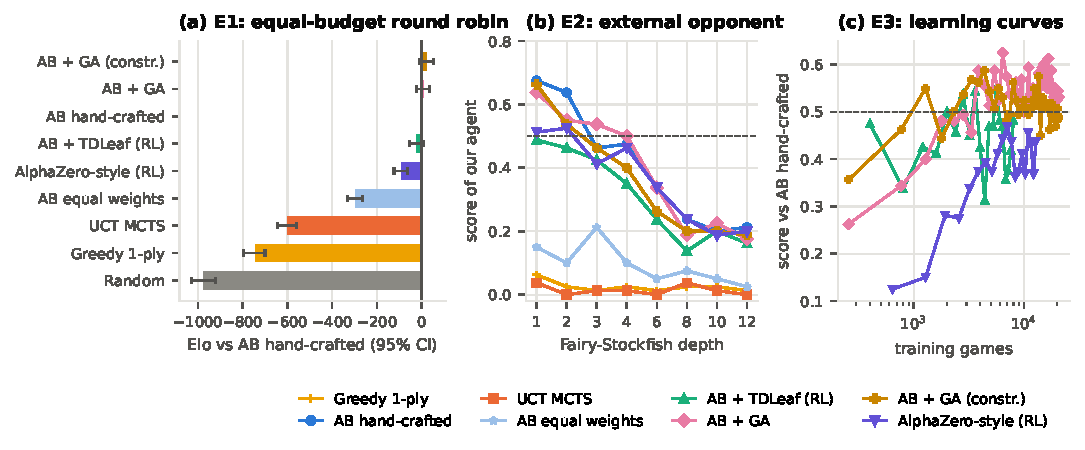
\includegraphics[width=\textwidth]{fig_report_a.pdf}
\caption{(a) Elo of every agent at an equal budget of 400 nodes or simulations, relative to the hand-crafted alpha-beta agent (bars: Bradley--Terry fit, whiskers: 95\% bootstrap interval; 120 games per pairing). (b) Score against Fairy-Stockfish at fixed depth (40 games per point; 0.5 = parity). (c) Score of each saved training checkpoint against the hand-crafted agent (same protocol).}
\label{fig:a}
\end{figure*}

\begin{table}[t]
\caption{Equal-budget results ($B=400$). Elo from the round robin; score against the hand-crafted agent; time per move; mean evaluation loss and blunder rate (loss $\ge200$ cp) from E4 (300 positions).}
\label{tab:main}
\centering
\small
\setlength{\tabcolsep}{3pt}
\resizebox{\columnwidth}{!}{%
\begin{tabular}{lcccrr}
\toprule
Agent & Elo [95\% CI] & vs hand & ms/move & loss (cp) & blund. \\
\midrule
Alpha-beta + GA (constr.) & +23 [-10, +53] & 0.53 & 0.2 & 61 & 9\% \\
Alpha-beta + GA & +7 [-24, +37] & 0.53 & 0.19 & 66 & 10\% \\
Alpha-beta, hand-crafted & +0 [+0, +0] & -- & 0.19 & 73 & 11\% \\
Alpha-beta + TDLeaf (RL) & -24 [-54, +7] & 0.44 & 0.2 & 83 & 13\% \\
AlphaZero-style (RL) & -90 [-123, -63] & 0.43 & 2.3 & 143 & 21\% \\
Alpha-beta, equal weights & -296 [-333, -265] & 0.13 & 0.2 & 125 & 19\% \\
UCT MCTS & -598 [-643, -558] & 0.02 & 5.7 & 386 & 50\% \\
Greedy 1-ply & -744 [-797, -700] & 0.01 & 0.013 & 260 & 34\% \\
Random & -973 [-1029, -921] & 0.00 & 0.009 & 612 & 71\%
\\
\bottomrule
\end{tabular}}
\end{table}

\textbf{E1, equal budget.} The four alpha-beta agents with a sensible evaluation (hand-crafted, TDLeaf, GA, constrained GA) are within 47 Elo of each other and their intervals overlap (about $\pm$32 Elo), so we cannot rank them. The AlphaZero-style agent is $-$90 Elo below the hand-crafted agent (95\% interval $-$123 to $-$63; score 0.43 against it, W28 D47 L45), the equal-weight agent is $-$296, and UCT MCTS is $-$598. TDLeaf starts from equal piece values and no positional knowledge, which is the equal-weight agent; the \emph{learned} weights are worth +272 Elo more. The GA, which starts from random weights, ends at +7 (unconstrained) and +23 (constrained).

\textbf{Cost.} A simulation of the network agent is much more expensive than an alpha-beta node: 2.3 ms against 0.19 ms per move at $B=400$. When alpha-beta is given the 6\,300 nodes it can search in the same time, the network agent scores only 0.25 against it (W12 D36 L72); at that budget alpha-beta reaches depth 4.0 instead of 1.8. UCT MCTS needs 5.7 ms per move and still scores 0.00 against time-matched alpha-beta.

\textbf{E2, external opponent.} (Fig.~\ref{fig:a}b.) The hand-crafted, GA and constrained-GA agents score 0.54--0.68 against Fairy-Stockfish at depths 1--2, hold roughly parity at depths 3--4 and score about 0.17--0.23 at depths 10--12. The AlphaZero-style and TDLeaf agents follow the same curve somewhat lower at shallow depth. The equal-weight agent averages 0.14 over depths 1--4 and the TDLeaf agent trained from it 0.43 (hand-crafted: 0.56); MCTS and the greedy agent score at most 0.06 even at depth 1.

\textbf{E3, learning curves.} (Fig.~\ref{fig:a}c.) All three learners start far below the hand-crafted agent and climb towards it. TDLeaf goes from 0.06 (equal weights) to about 0.45 within roughly 2400 games and then fluctuates; the GA climbs from 0.26 to about 0.55 within 4000 fitness games; the network agent rises from 0.12 to about 0.41 after roughly 7000 self-play games and then stays flat (policy loss 1.37). None settles above about 0.6.

\textbf{E4, move quality.} (Table~\ref{tab:main}.) The constrained GA, GA and hand-crafted agents lose 61, 66 and 73 cp per move and TDLeaf 83; their paired differences from the hand-crafted agent have bootstrap intervals that include zero. The equal-weight agent loses 125 cp and the AlphaZero-style agent 143 cp (70 cp more than hand-crafted, 95\% interval 36 to 103); its blunder rate is 21\% against 11\%.

\textbf{Learned weights and scaling.} (Fig.~\ref{fig:b}.) TDLeaf values knight, bishop, rook and queen at 2.4, 2.2, 3.8 and 4.9 pawns (hand-crafted: 3, 3.2, 5, 9); the unconstrained GA at 1.4, 1.3, 1.9 and 2.6. The order is right but the scale is compressed. Strength grows with budget for every agent: the network agent gains from $-$199 to +70 Elo between 25 and 1600 simulations (measured against alpha-beta at 400 nodes), and alpha-beta with the GA weights reaches 0.78 points at 1600 nodes; MCTS stays below 0.07 points against that opponent and is omitted from the plot.

\begin{figure*}[t]
\centering
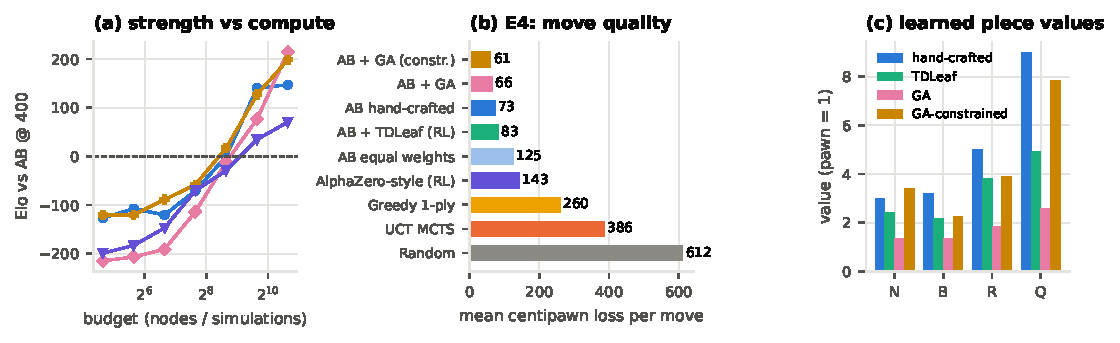
\includegraphics[width=\textwidth]{fig_report_b.pdf}
\caption{(a) Score-derived Elo against alpha-beta at 400 nodes as a function of budget (60 games per point; UCT MCTS stays below $-400$ and is omitted). (b) Mean centipawn loss per move against Fairy-Stockfish depth 9 on 300 positions. (c) Piece values learned by TDLeaf and by the two genetic algorithms, relative to the pawn.}
\label{fig:b}
\end{figure*}

\section{Discussion}
\textbf{Learning recovers, but does not exceed, expert knowledge.} Two methods that were given no chess knowledge end close to a hand-written evaluation: the GA, from game scores inside its population, and TDLeaf, from the result signal (somewhat lower than the hand-crafted agent against the outside engine at shallow depth); the network agent, trained on search statistics, ends further behind. The GA and TDLeaf match the hand-crafted agent in move quality (E4). The learned piece values are smaller than the textbook ones. The GA tuned its weights at 400 nodes, where alpha-beta reaches depth about 1.8 (mean over our E4 positions), so part of what they encode may be a correction for shallow search; TDLeaf trained with depth-3 search. We did not test this, or the effect of board size.

\textbf{Why the AlphaZero-style agent is behind.} With 12\,800 games and a 216\,000-parameter perceptron, the network is a weaker evaluator than 14 hand-chosen features combined with exact tactics from quiescence search; its losses stop decreasing early, which suggests a limit of data or capacity rather than of training time, but we did not vary either. Its scaling curve is the steepest, so it is not hopeless, but each simulation costs about 12 nodes. The result should not be read as a statement about AlphaZero at scale.

\textbf{UCT MCTS} is limited by random rollouts: in a tactical game a single blunder decides the result, so value estimates are noisy and our budgets are small.

\textbf{A validity lesson.} In an earlier version of the harness both sides of a game shared one transposition table, so an agent could reuse scores computed with the other agent's weights. In that version the unconstrained GA scored 0.74 against the hand-crafted agent at 2000 nodes (now 0.48), and the AlphaZero-style agent looked like the strongest one. The inconsistency showed up only against Fairy-Stockfish: an agent that beat the hand-crafted one head to head scored near zero from depth 4. Each side now owns its table, and every number here was produced after the fix. Without an external opponent we might not have seen it.

\section{Inference}
The evidence supports: (1) game results alone are enough for TDLeaf to move an equal-weight evaluation by +272 Elo to hand-crafted level, and a GA reaches the same level from random weights; no learner is shown to be better than the hand-written weights, since all intervals overlap; (2) at this data and compute scale a search with a linear evaluation beats a small self-play network both at equal budget and at equal time, and UCT with random rollouts is far weaker; (3) the in-pool ranking agrees with an independent engine and with move-level analysis, which is why we trust it. It does not support: differences smaller than about $\pm$32 Elo; claims about seeds, since each learner was trained once; claims about larger networks, longer training, or other variants. The E4 positions and Fairy-Stockfish depth are proxies, not a calibrated Elo.

\section{Conclusion}
We compared five techniques for Gardner minichess on one engine under one compute currency. With the same alpha-beta search, an evaluation learned by TDLeaf or evolved by a GA from no knowledge reaches the level of a hand-written one; an AlphaZero-style network trained for 35 CPU-minutes does not, and costs more per simulation; random-rollout MCTS is far behind. External play against Fairy-Stockfish was essential to detect a harness error. Next steps are repeated seeds with confidence bands, GA fitness that includes an outside opponent or a hall of fame \cite{rosin1997}, convolutional networks with search-value targets, and the Silverman $4\times5$ and Los Alamos $6\times6$ variants to test transfer. Code, data and the interactive board are in the project repository.
